\noindent
\graphicspath{{./15-07/Images/}} 
%%%%%%%%%%%%%%%%
% Page de gauche
%%%%%%%%%%%%%%%%
\begin{minipage}[t][\textheight][t]{0.33\textwidth}
    \colorbox{StrongBlue}{
        \parbox[c][\textheight][c]{\textwidth}{ 
            \color{OffWhite} 
            \begin{center}
                \noindent
                \begin{minipage}[t][0.55\textheight][c]{0.8\textwidth}
                    {\huge \textbf{Mercredi 15 Juillet}}\\
                    \normalsize
                    \begin{center}
                        \begin{tabular}{@{} l @{\hspace{0.5cm}} l @{}}
                            Abri de départ : &\hfill Pornic \\ 
                            Abri d'arrivée : &\hfill Pornichet \\ 
                            Distance : &\hfill 17 Milles \\
                            Durée : &\hfill 4 Heures 30 \\ 
                            Départ : &\hfill 9 h 30 \\ 
                            Arrivée prévue : &\hfill 16 h 30 \\ 
                            Lever soleil 
\includegraphics[width=8px,height=8px]{../../Pictos/soleil_OffWhite.png}
 : &\hfill 06 h 28 \\ 
                            Coucher soleil 
\includegraphics[width=8px,height=8px]{../../Pictos/lune_OffWhite.png} : &\hfill 22 h 00 \\ 
                            \\
                            Abris replis : &  \\
                                    & • Pornic \\
                                    & • Port de la Gravette  \\
                                    & • Pornichet \\                    
                                
                        \end{tabular}
                    \end{center}
                    
                \end{minipage}%

                \begin{minipage}[t][0.4\textheight][t]{\textwidth}

                    \begin{center}
    {\large \textit{Marées \textbf{Pornic}}}\\ \vspace{0.5em}
    
    \renewcommand{\arraystretch}{1.40}
    
    \begin{tabular}{ |C{5em}|c|C{4em}|C{4em}|}\hline
        & Coef & Heure & Hauteur\\ \hline
        BM & \multirow{2}{1em}{94} & 00 h 03 & 0,94 m\\ \cline{1-1} \cline{3-4} 
        PM & & 06 h 18 & 5,69 m\\\hline 
        BM & \multirow{2}{1em}{96} & 12 h 18 & 1,07 m\\ \cline{1-1} \cline{3-4} 
        PM &  & 18 h 16 & 6,02 m\\ \hline
    \end{tabular}
    % \textit{Le port de \textbf{Pornichet} est décalé de 5 minutes}

\end{center}
                    \begin{center}
    {\large \textit{Marées \textbf{Pornichet}}}\\ \vspace{0.5em}
    
    \renewcommand{\arraystretch}{1.40}
    
    \begin{tabular}{ |C{5em}|c|C{4em}|C{4em}|}\hline
        & Coef & Heure & Hauteur\\ \hline
        PM & 94 & 06 h 04 & 5,42 m\\ \hline
        BM & \multirow{2}{1em}{96} & 12 h 12 & 0,78 m\\ \cline{1-1} \cline{3-4} 
        PM &   & 18 h 11 & 5,67 m\\ \hline
    \end{tabular}
\end{center}
                \end{minipage}%
            \end{center}       
        }      
    }
\end{minipage}%
\begin{minipage}[c][\textheight][t]{0.10\textwidth}
\hfill
\end{minipage}%
\begin{minipage}[c][\textheight][t]{0.50\textwidth}
    \vspace{2.5cm}
    \color{StrongBlue}    
    {\huge \textbf{Description de la navigation}}\\
            \vspace{0.1cm}\\
            {\large \textbf{Sortie de Pornic}}\\
            \begin{itemize}
                \itemsep0em 
                \item Départ de Pornic à 9h30 h après une prise en main des bateaux par les équipages. Attention à bien respecter le chenal et à ne pas border les balises latérales tribord. Présence de rochers.
                \item Le chenal du port de Pornic à une sonde à 0.7m, le tirant d'eau maximale de la flotte étant de 1.45, on s'assurera d'avoir au moins 1.3m d'eau de hauteure d'eau pour sortir du port : \textbf{les bateaux doivent donc impérativement avoir quitté le chenal à 11h15}. 
                \item Une fois sortis du chenal, hisser les voiles.

            \end{itemize}
            {\large \textbf{Déroulé de la navigation}}\\
            \begin{itemize}
                \itemsep0em 
                \item Prendre la direction de la marque spéciale qu'on laissera à notre Nord. Longer ensuite la côte jusqu'à la pointe de saint Gildas. La côte est relativement franche. 
                \item Au niveau de la pointe de st Gildas, s'éloigner largement pour éviter les rochers. Prendre un cap à 320 en direction du Grand charpentier. 
                \item Attention à ne pas se rapprocher de la cardinale Nord Couronnée.
                \item Pour éviter le plateau de la lambarde on peut viser les bouées babord n°2 tribord n°1 du chenal de st nazaire et les laisser à notre babord. A cet endroit dégagé on pourra manger à la cap en séparant les deux flotilles. La marée sera montante sur son premier douzième donc peu de risques. 
                \item Après le repas on pourra rectifier le cap en fonction de la dérive en direction de l'entrée des Troves.
                \item On veillera à laisser le Grand Charpentier et la Pierre percée largement à notre tribord. 
                \item Entrée via la passe des Troves une fois qu'elle est dans notre 45°, attention à ne pas la border, ses abords ne sont pas francs, le bateau CF ouvre la marche. 
            \end{itemize}
        
        {\large \textbf{Arrivée à Pornichet}}\\
            \begin{itemize}
                \itemsep0em 
                \item Une fois les Troves passées, cap vers Pornichet, affalage devant la jetée. 
                \item Ne pas aller trop en avant dans la baie (rocher des Troves)
                \item C'est la première journée de navigation du camp, on ne manquera pas de s'assurer de l'état des troupes à l'arrivée.
            \end{itemize}
\end{minipage}%
%%%%%%%%%%%%%%%%
% Page de droite
%%%%%%%%%%%%%%%%
\newgeometry{top=2cm, bottom=2cm, left=2cm, right=2cm}
\begin{minipage}[t][0.9\textheight][t]{0.60\textwidth}
    \color{StrongBlue}    
    \noindent
    \begin{minipage}[t][0.3\textheight][t]{\textwidth}
        \begin{minipage}[t][0.3\textheight][t]{0.65\textwidth}
            \vspace{-8.5em}
            {\huge \textbf{Détails de la navigation}}\\
            Le QR-code situé à droite est cliquable, il permet d'explorer le planning de navigation sur le site datashom. 
            La carte ci-dessous visualise le trajet prévu ainsi que les abris de replis et dangers identifiés. 
        \end{minipage}%
        \hfill
        \begin{minipage}[t][0.3\textheight][t]{0.25\textwidth}       
        \href{https://data.shom.fr/datacontext/fr/1780678005523-480815}{ 
            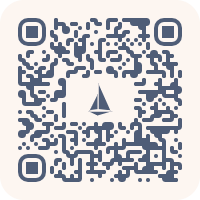
\includegraphics[width=0.8\textwidth]{qr-code.png}
        }
        \end{minipage}%
    \end{minipage}
        \begin{minipage}[t][0.7\textheight][t]{\textwidth}
        % 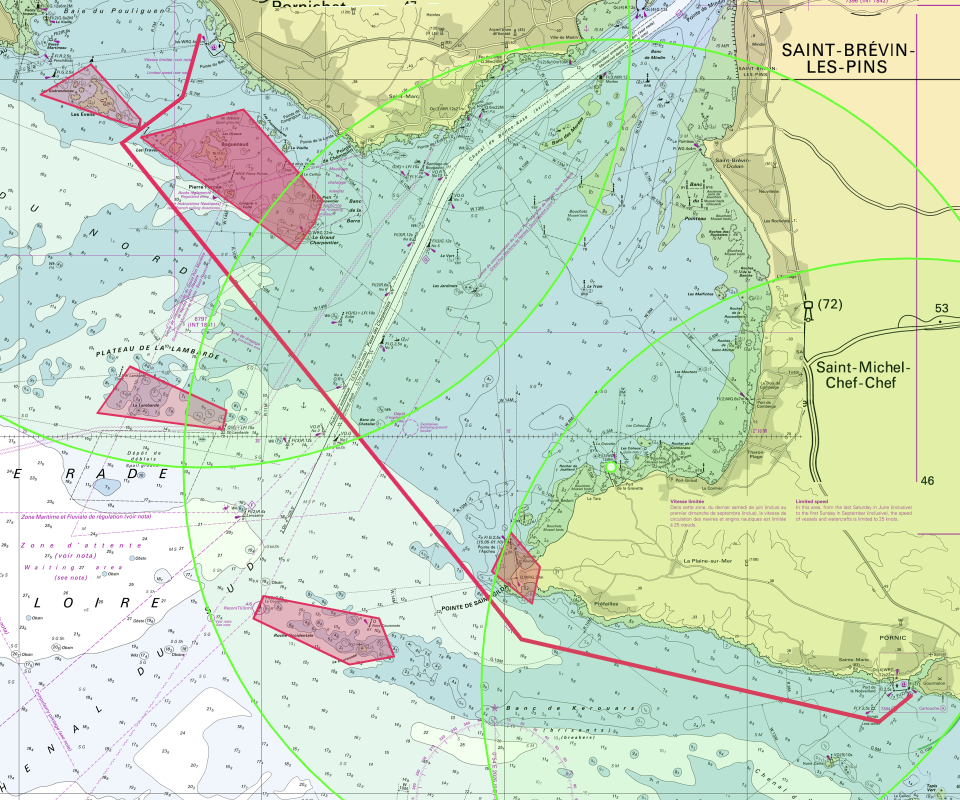
\includegraphics[width=0.97\textwidth]{carte.png}
        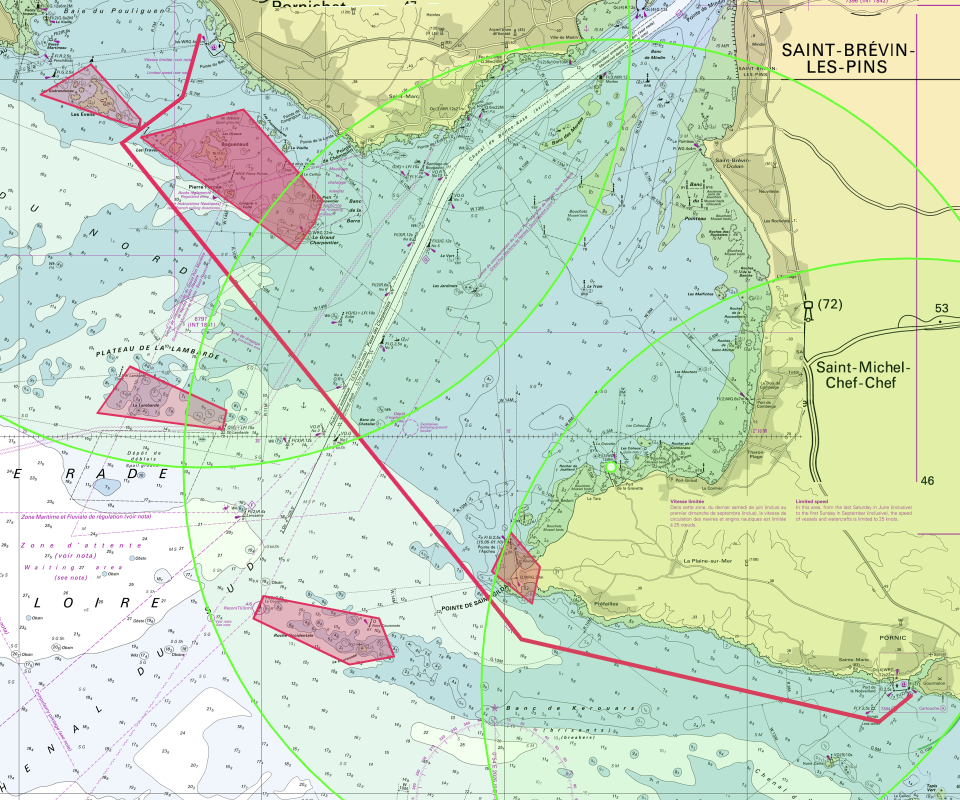
\includegraphics[height=0.7\textheight]{carte.png}
    \end{minipage}
\end{minipage}
\begin{minipage}[t][0.9\textheight][t]{0.40\textwidth}
    \color{StrongBlue} 
    \centering 
    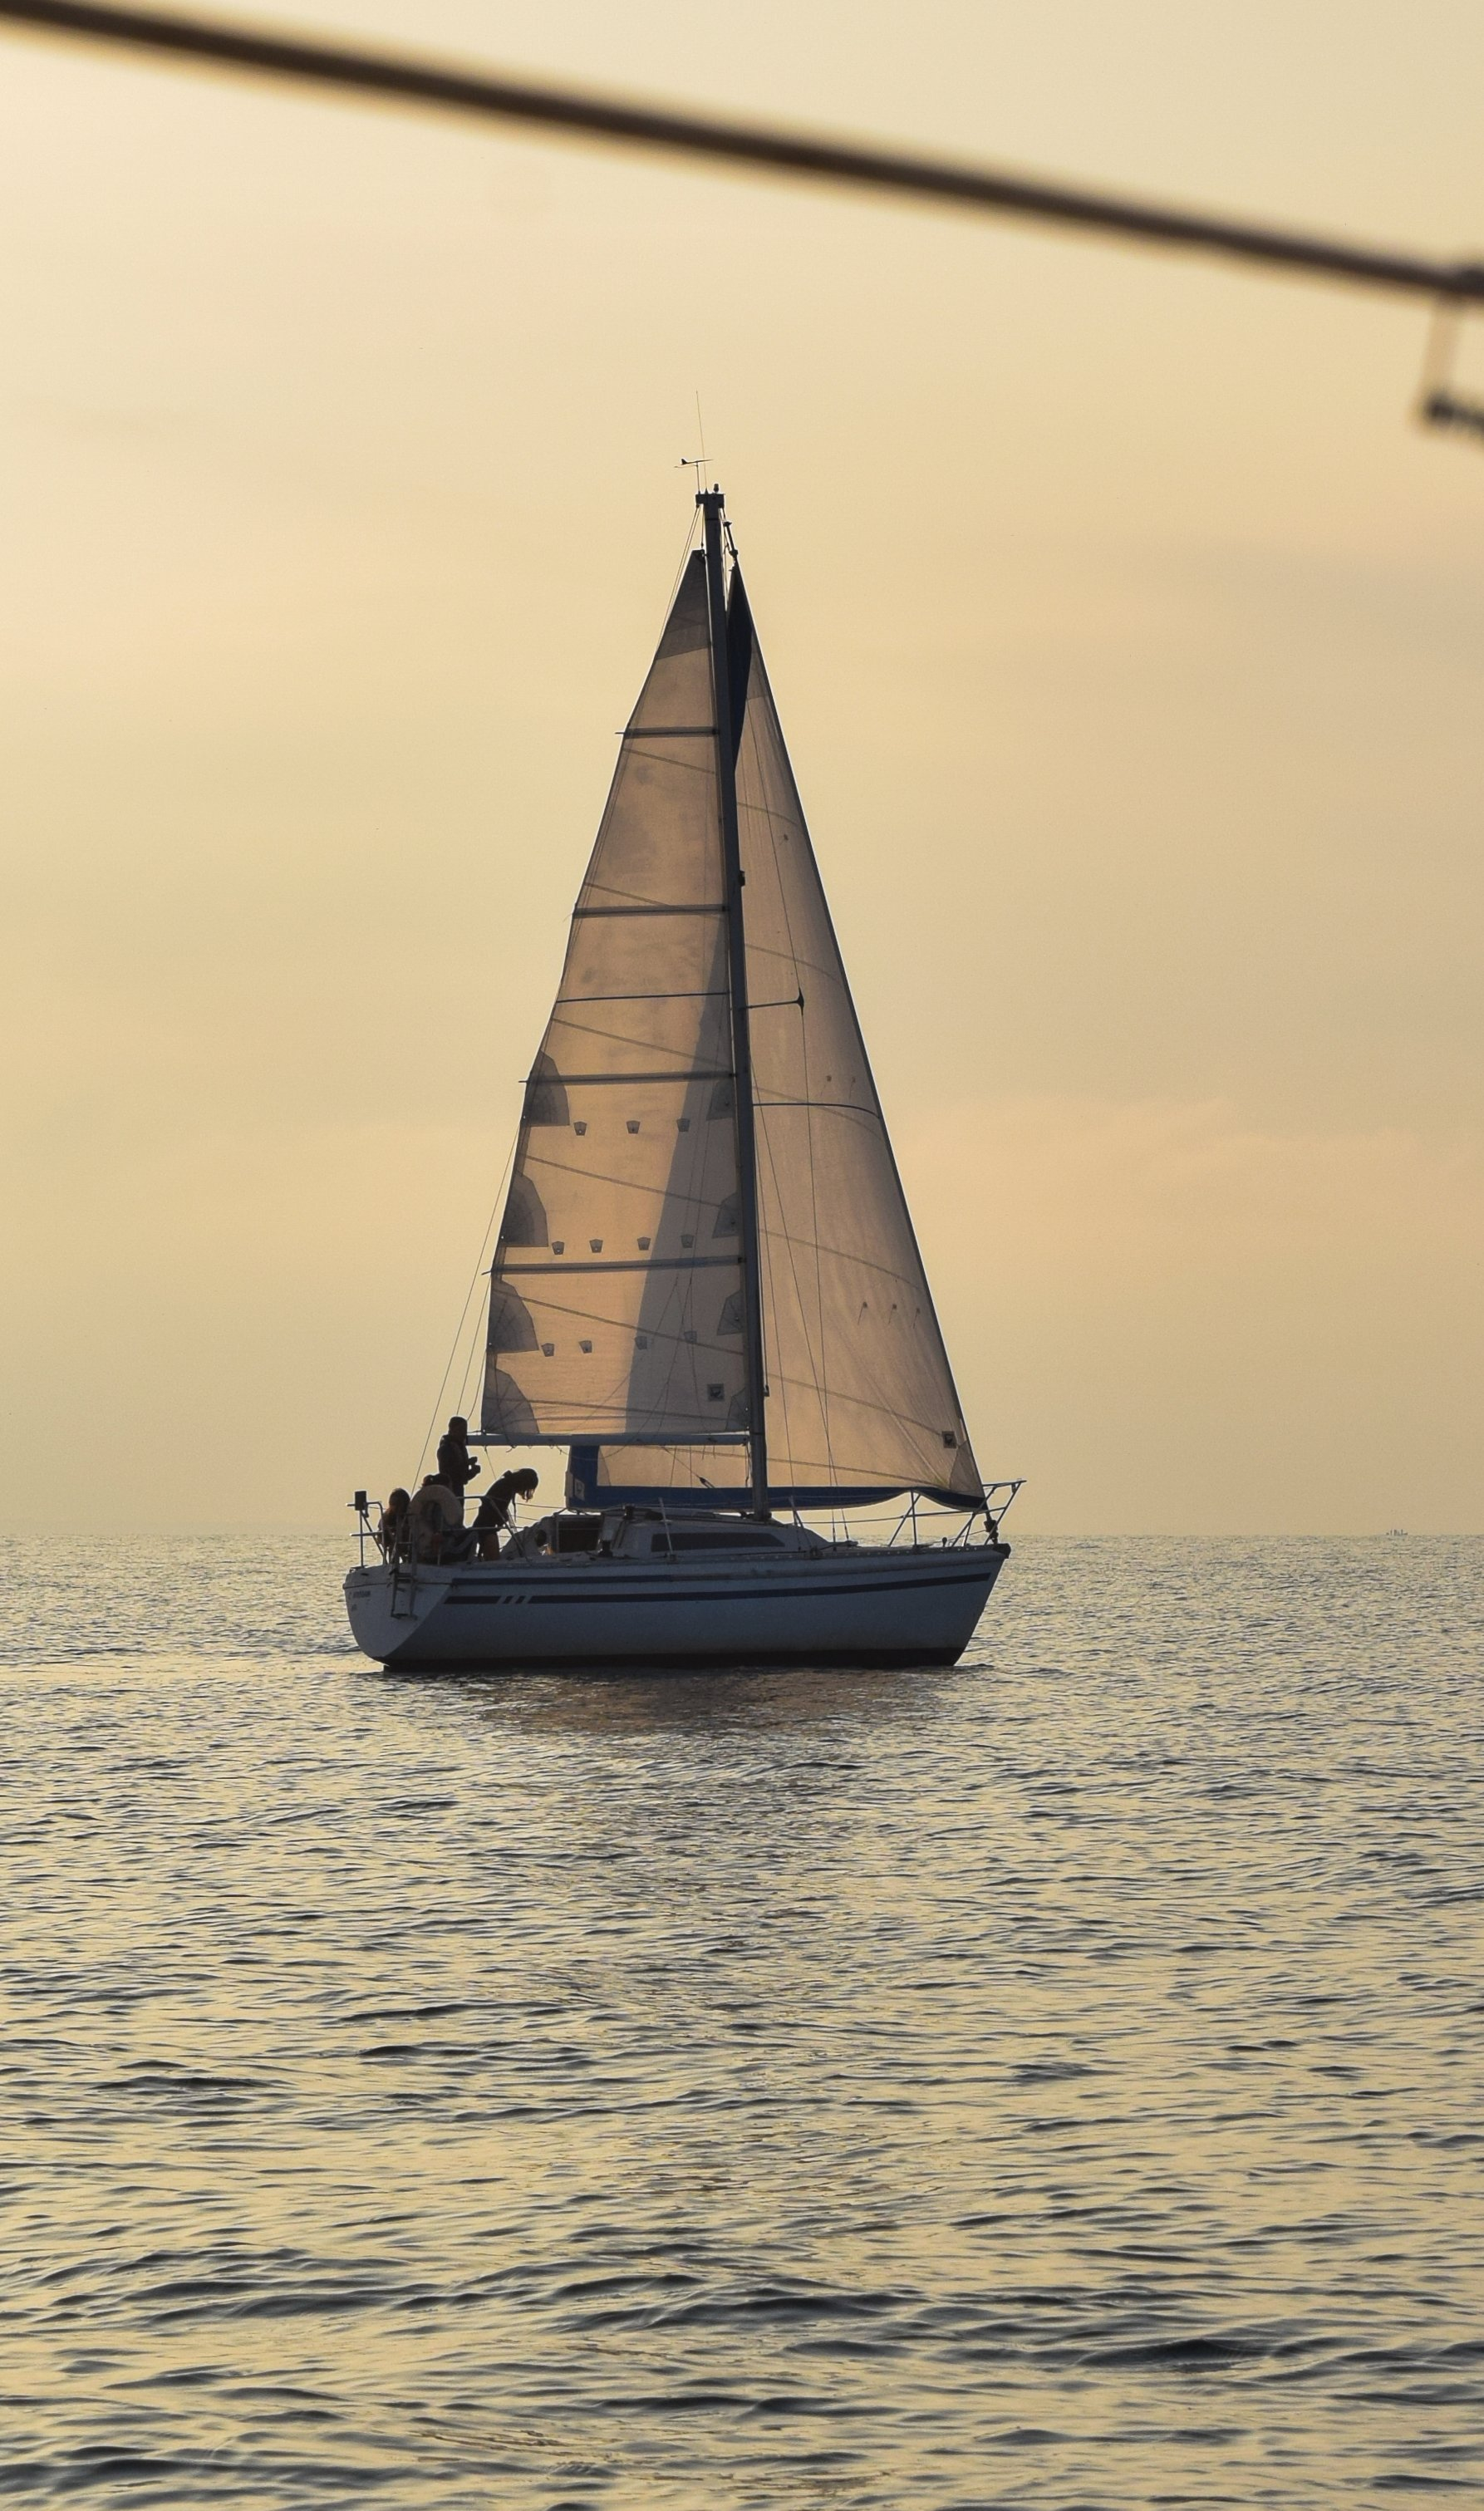
\includegraphics[height=\textheight, width=\textwidth, keepaspectratio]{illustration_verticale.jpg}
\end{minipage}%
\restoregeometry



